% This article has been prepared for publication in Energy Economics in RStudio with knitr.
% According to http://www.elsevier.com/author-schemas/the-elsarticle-latex-document-class, we should be using the
% elsarticle.cls file.
% According to http://cdn.elsevier.com/assets/pdf_file/0006/109392/journal_refstyles.pdf, we should be using
% elsarticle-template-2-harv.tex as the template for the text.
% Furthermore, we should be using model2-names.bst for the bibliographic references.
% The approach here is to load the frontmatter and backmatter from elsarticle-template-2-harv.tex
% both ahead of and behind the text for our paper.
% -- Matthew Kuperus Heun, 2013-01-18

%% This is file `elsarticle-template-2-harv.tex',
%%
%% Copyright 2009 Elsevier Ltd
%%
%% This file is part of the 'Elsarticle  Bundle'.
%% ---------------------------------------------
%%
%% It may be distributed under the conditions of the LaTeX Project Public
%% License, either version 1.2 of this license or (at your option) any
%% later version.  The latest version of this license is in
%%    http://www.latex-project.org/lppl.txt
%% and version 1.2 or later is part of all distributions of LaTeX
%% version 1999/12/01 or later.
%%
%% The list of all files belonging to the 'Elsarticle Bundle' is
%% given in the file `manifest.txt'.
%%
%% Template article for Elsevier's document class `elsarticle'
%% with harvard style bibliographic references
%%
%% $Id: elsarticle-template-2-harv.tex 155 2009-10-08 05:35:05Z rishi $
%% $URL: http://lenova.river-valley.com/svn/elsbst/trunk/elsarticle-template-2-harv.tex $
%%
\documentclass[preprint,authoryear,12pt]{elsarticle}\usepackage{graphicx, color}
%% maxwidth is the original width if it is less than linewidth
%% otherwise use linewidth (to make sure the graphics do not exceed the margin)
\makeatletter
\def\maxwidth{ %
  \ifdim\Gin@nat@width>\linewidth
    \linewidth
  \else
    \Gin@nat@width
  \fi
}
\makeatother

\IfFileExists{upquote.sty}{\usepackage{upquote}}{}
\definecolor{fgcolor}{rgb}{0.2, 0.2, 0.2}
\newcommand{\hlnumber}[1]{\textcolor[rgb]{0,0,0}{#1}}%
\newcommand{\hlfunctioncall}[1]{\textcolor[rgb]{0.501960784313725,0,0.329411764705882}{\textbf{#1}}}%
\newcommand{\hlstring}[1]{\textcolor[rgb]{0.6,0.6,1}{#1}}%
\newcommand{\hlkeyword}[1]{\textcolor[rgb]{0,0,0}{\textbf{#1}}}%
\newcommand{\hlargument}[1]{\textcolor[rgb]{0.690196078431373,0.250980392156863,0.0196078431372549}{#1}}%
\newcommand{\hlcomment}[1]{\textcolor[rgb]{0.180392156862745,0.6,0.341176470588235}{#1}}%
\newcommand{\hlroxygencomment}[1]{\textcolor[rgb]{0.43921568627451,0.47843137254902,0.701960784313725}{#1}}%
\newcommand{\hlformalargs}[1]{\textcolor[rgb]{0.690196078431373,0.250980392156863,0.0196078431372549}{#1}}%
\newcommand{\hleqformalargs}[1]{\textcolor[rgb]{0.690196078431373,0.250980392156863,0.0196078431372549}{#1}}%
\newcommand{\hlassignement}[1]{\textcolor[rgb]{0,0,0}{\textbf{#1}}}%
\newcommand{\hlpackage}[1]{\textcolor[rgb]{0.588235294117647,0.709803921568627,0.145098039215686}{#1}}%
\newcommand{\hlslot}[1]{\textit{#1}}%
\newcommand{\hlsymbol}[1]{\textcolor[rgb]{0,0,0}{#1}}%
\newcommand{\hlprompt}[1]{\textcolor[rgb]{0.2,0.2,0.2}{#1}}%

\usepackage{framed}
\makeatletter
\newenvironment{kframe}{%
 \def\at@end@of@kframe{}%
 \ifinner\ifhmode%
  \def\at@end@of@kframe{\end{minipage}}%
  \begin{minipage}{\columnwidth}%
 \fi\fi%
 \def\FrameCommand##1{\hskip\@totalleftmargin \hskip-\fboxsep
 \colorbox{shadecolor}{##1}\hskip-\fboxsep
     % There is no \\@totalrightmargin, so:
     \hskip-\linewidth \hskip-\@totalleftmargin \hskip\columnwidth}%
 \MakeFramed {\advance\hsize-\width
   \@totalleftmargin\z@ \linewidth\hsize
   \@setminipage}}%
 {\par\unskip\endMakeFramed%
 \at@end@of@kframe}
\makeatother

\definecolor{shadecolor}{rgb}{.97, .97, .97}
\definecolor{messagecolor}{rgb}{0, 0, 0}
\definecolor{warningcolor}{rgb}{1, 0, 1}
\definecolor{errorcolor}{rgb}{1, 0, 0}
\newenvironment{knitrout}{}{} % an empty environment to be redefined in TeX

\usepackage{alltt}

%% Use the option review to obtain double line spacing
%% \documentclass[authoryear,preprint,review,12pt]{elsarticle}

%% Use the options 1p,twocolumn; 3p; 3p,twocolumn; 5p; or 5p,twocolumn
%% for a journal layout:
%% \documentclass[final,authoryear,1p,times]{elsarticle}
%% \documentclass[final,authoryear,1p,times,twocolumn]{elsarticle}
%% \documentclass[final,authoryear,3p,times]{elsarticle}
%% \documentclass[final,authoryear,3p,times,twocolumn]{elsarticle}
%% \documentclass[final,authoryear,5p,times]{elsarticle}
%% \documentclass[final,authoryear,5p,times,twocolumn]{elsarticle}

%% if you use PostScript figures in your article
%% use the graphics package for simple commands
%% \usepackage{graphics}
%% or use the graphicx package for more complicated commands
%% \usepackage{graphicx}
%% or use the epsfig package if you prefer to use the old commands
%% \usepackage{epsfig}

%% The amssymb package provides various useful mathematical symbols
\usepackage{amssymb}
%% The amsthm package provides extended theorem environments
%% \usepackage{amsthm}

%% The lineno packages adds line numbers. Start line numbering with
%% \begin{linenumbers}, end it with \end{linenumbers}. Or switch it on
%% for the whole article with \linenumbers after \end{frontmatter}.
%% \usepackage{lineno}

%% natbib.sty is loaded by default. However, natbib options can be
%% provided with \biboptions{...} command. Following options are
%% valid:

%%   round  -  round parentheses are used (default)
%%   square -  square brackets are used   [option]
%%   curly  -  curly braces are used      {option}
%%   angle  -  angle brackets are used    <option>
%%   semicolon  -  multiple citations separated by semi-colon (default)
%%   colon  - same as semicolon, an earlier confusion
%%   comma  -  separated by comma
%%   authoryear - selects author-year citations (default)
%%   numbers-  selects numerical citations
%%   super  -  numerical citations as superscripts
%%   sort   -  sorts multiple citations according to order in ref. list
%%   sort&compress   -  like sort, but also compresses numerical citations
%%   compress - compresses without sorting
%%   longnamesfirst  -  makes first citation full author list
%%
%% \biboptions{longnamesfirst,comma}

% \biboptions{}

\journal{Energy Economics}

\begin{document}

\begin{frontmatter}

%% Title, authors and addresses

%% use the tnoteref command within \title for footnotes;
%% use the tnotetext command for the associated footnote;
%% use the fnref command within \author or \address for footnotes;
%% use the fntext command for the associated footnote;
%% use the corref command within \author for corresponding author footnotes;
%% use the cortext command for the associated footnote;
%% use the ead command for the email address,
%% and the form \ead[url] for the home page:
%%
%% \title{Title\tnoteref{label1}}
%% \tnotetext[label1]{}
%% \author{Name\corref{cor1}\fnref{label2}}
%% \ead{email address}
%% \ead[url]{home page}
%% \fntext[label2]{}
%% \cortext[cor1]{}
%% \address{Address\fnref{label3}}
%% \fntext[label3]{}

\title{Empirical Analysis of the Role of Energy in Economic Growth}

%% use optional labels to link authors explicitly to addresses:
%% \author[label1,label2]{<author name>}
%% \address[label1]{<address>}
%% \address[label2]{<address>}

\author[Calvin]{Caleb Reese}
\author[Calvin]{Lucas Timmer}
\author[Calvin]{Matthew Kuperus Heun\corref{cor1}}
\ead{mkh2@calvin.edu, tel: +1 (616) 526-6663, fax: +1 (616) 526-6501}

\cortext[cor1]{Corresponding author}
\address[Calvin]{Engineering Department, Calvin College, Grand Rapids, MI 49546, USA}

\begin{abstract}
%% Text of abstract
*********** Add abstract ***********
\end{abstract}

\begin{keyword}
%% keywords here, in the form: keyword \sep keyword
economic growth \sep energy \sep cobb-douglas \sep CES \sep LINEX
%% MSC codes here, in the form: \MSC code \sep code
%% or \MSC[2008] code \sep code (2000 is the default)
\end{keyword}

\end{frontmatter}

% \linenumbers
%% main text

Caleb, put your LaTeX code here.












\section{Cobb-Douglas Without Energy}

\begin{knitrout}
\definecolor{shadecolor}{rgb}{0.969, 0.969, 0.969}\color{fgcolor}\begin{kframe}
\begin{verbatim}
[1] "US"
    pred
1  1.000
2  1.020
3  1.026
4  1.057
5  1.119
6  1.161
7  1.196
8  1.244
9  1.296
10 1.348
11 1.375
12 1.383
13 1.408
14 1.458
15 1.520
16 1.579
17 1.628
18 1.702
19 1.772
20 1.844
21 1.912
22 1.940
23 1.963
24 1.997
25 2.058
26 2.128
27 2.204
28 2.260
29 2.280
30 2.214
31 2.241
32 2.323
[1] "UK"
     pred
1  1.0000
2  0.9791
3  0.9841
4  1.0027
5  1.0325
6  1.0868
7  1.1253
8  1.1719
9  1.2250
10 1.2865
11 1.3170
12 1.3292
13 1.3248
14 1.3535
15 1.3991
16 1.4403
17 1.5209
18 1.5508
19 1.5964
20 1.6428
21 1.6781
22 1.7411
23 1.7699
24 1.8196
25 1.8725
26 1.9292
27 1.9699
28 1.9903
29 2.0312
30 2.0002
31 2.0666
32 2.0676
[1] "JP"
    pred
1  1.000
2  1.037
3  1.077
4  1.118
5  1.144
6  1.177
7  1.216
8  1.256
9  1.306
10 1.356
11 1.406
12 1.455
13 1.495
14 1.515
15 1.543
16 1.577
17 1.614
18 1.639
19 1.648
20 1.648
21 1.672
22 1.679
23 1.680
24 1.699
25 1.719
26 1.737
27 1.762
28 1.781
29 1.786
30 1.761
31 1.762
32 1.749
[1] "CN"
    pred
1  1.000
2  1.096
3  1.223
4  1.365
5  1.519
6  1.685
7  1.859
8  2.054
9  2.255
10 2.483
11 2.708
12 2.979
13 3.296
14 3.619
15 4.008
16 4.443
17 4.917
18 5.424
19 6.061
20 6.769
21    NA
[1] "ZA"
    pred
1  1.000
2  1.018
3  1.024
4  1.081
5  1.103
6  1.126
7  1.193
8  1.181
9  1.223
10 1.257
11 1.282
12 1.284
13 1.358
14 1.434
15 1.458
16 1.523
17 1.605
18 1.686
19 1.701
20 1.772
21    NA
[1] "SA"
    pred
1  1.000
2  1.040
3  1.067
4  1.089
5  1.094
6  1.107
7  1.104
8  1.114
9  1.132
10 1.156
11 1.193
12 1.230
13 1.297
14 1.363
15 1.410
16 1.464
17 1.529
18 1.614
19 1.622
20 1.620
21 1.790
[1] "IR"
    pred
1  1.000
2  1.018
3  1.045
4  1.055
5  1.072
6  1.091
7  1.141
8  1.187
9  1.229
10 1.293
11 1.354
12 1.424
13 1.516
14 1.629
15 1.711
16 1.774
17 1.856
18 1.894
19 1.982
20 2.072
21 2.156
[1] "TZ"
    pred
1  1.000
2  1.057
3  1.110
4  1.135
5  1.163
6  1.200
7  1.212
8  1.266
9  1.312
10 1.349
11 1.436
12 1.517
13 1.585
14 1.673
15 1.792
16 1.899
17 2.078
18 2.223
19 2.380
20 2.569
21 2.757
[1] "ZM"
    pred
1  1.000
2  1.016
3  1.013
4  1.007
5  1.026
6  1.038
7  1.099
8  1.140
9  1.204
10 1.230
11 1.279
12 1.325
13 1.380
14 1.425
15 1.494
16 1.578
17 1.639
18 1.713
19 1.815
20 1.914
21 2.055
\end{verbatim}
\end{kframe}
\end{knitrout}


% latex table generated in R 2.15.2 by xtable 1.7-0 package
% Sun Feb  3 21:37:31 2013
\begin{table}[ht]
\begin{center}
\caption{Cobb-Douglas (without energy) for 1980-2011 (US, UK, JP) or 1991-2011 (others). (Parameter estimates beneath symbol. 95\% confidence interval bounds to left and right.)}
\begin{tabular}{r|ccc|ccc|ccc}
  \hline
 &   & $\lambda$ &   &   & $\alpha$ &   &   & $\beta$ &   \\ 
  \hline
US & 0.0087 & 0.0102 & 0.0116 & 0.21 & 0.27 & 0.34 & 0.66 & 0.73 & 0.79 \\ 
  UK & -0.0104 & 0.0097 & 0.0303 & -0.25 & 0.44 & 1.12 & -0.13 & 0.56 & 1.24 \\ 
  JP & 0.0021 & 0.0052 & 0.0082 & 0.44 & 0.52 & 0.59 & 0.41 & 0.48 & 0.56 \\ 
  CN & -0.0405 & 0.0188 & 0.0779 & 0.11 & 0.71 & 1.32 & -0.32 & 0.29 & 0.89 \\ 
  ZA & -0.0007 & 0.0008 & 0.0022 & 0.46 & 0.60 & 0.73 & 0.26 & 0.40 & 0.54 \\ 
  SA & -0.0159 & -0.0123 & -0.0087 & 0.21 & 0.45 & 0.68 & 0.32 & 0.55 & 0.78 \\ 
  IR & 0.0032 & 0.0039 & 0.0045 & 0.49 & 0.60 & 0.70 & 0.30 & 0.40 & 0.51 \\ 
  TZ & -0.0039 & 0.0015 & 0.0068 & 0.50 & 0.73 & 0.95 & 0.05 & 0.27 & 0.50 \\ 
  ZM & 0.0218 & 0.0249 & 0.0280 & 1.25 & 1.41 & 1.57 & -0.57 & -0.41 & -0.25 \\ 
   \hline
\end{tabular}
\end{center}
\end{table}






\begin{knitrout}
\definecolor{shadecolor}{rgb}{0.969, 0.969, 0.969}\color{fgcolor}\begin{kframe}


{\ttfamily\noindent\color{warningcolor}{Warning: step factor 0.00012207 reduced below 'minFactor' of 0.000244141}}

{\ttfamily\noindent\color{warningcolor}{Warning: step factor 0.00012207 reduced below 'minFactor' of 0.000244141}}

{\ttfamily\noindent\color{warningcolor}{Warning: step factor 0.00012207 reduced below 'minFactor' of 0.000244141}}

{\ttfamily\noindent\color{warningcolor}{Warning: step factor 0.00012207 reduced below 'minFactor' of 0.000244141}}\begin{verbatim}
[1] "predGDPQ"
\end{verbatim}


{\ttfamily\noindent\color{warningcolor}{Warning: step factor 0.00012207 reduced below 'minFactor' of 0.000244141}}

{\ttfamily\noindent\color{warningcolor}{Warning: step factor 0.00012207 reduced below 'minFactor' of 0.000244141}}\begin{verbatim}
[1] "predGDPX"
\end{verbatim}
\end{kframe}\begin{figure}[]

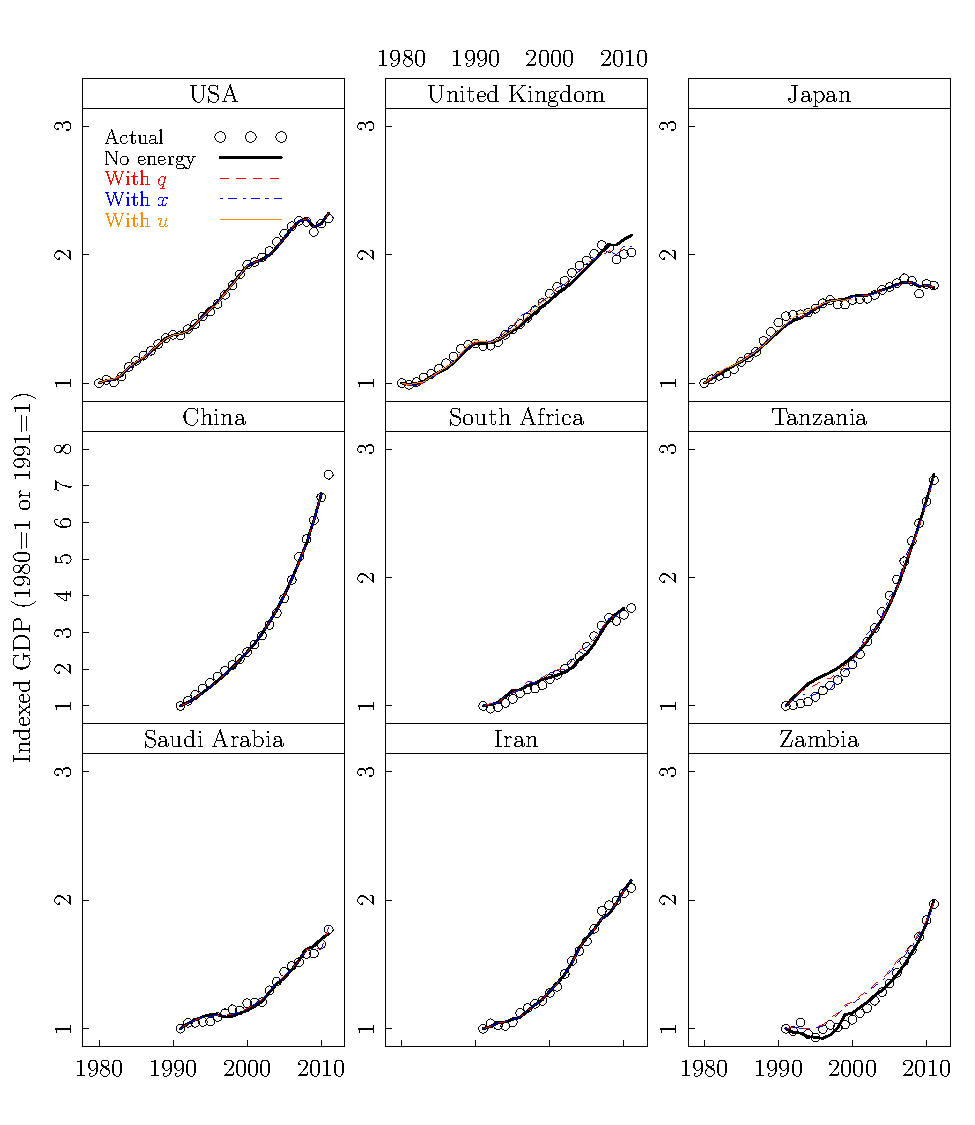
\includegraphics[width=\maxwidth]{figure/CD_GDP_Lattice_Graph} \caption[Cobb-Douglas results]{Cobb-Douglas results.\label{fig:CD_GDP_Lattice_Graph}}
\end{figure}


\end{knitrout}


\section{Cobb-Douglas With Energy}

We can force $\alpha$, $\beta$, and $\gamma$ to be in $[0,1]$ by a reparameterization:

\[ a \in[0,1], b \in [0,1], \alpha=\min(a,b), \beta=|b-a|, \gamma = 1-\max(a,b) \]




\subsection{Cobb-Douglas with $Q$}







\subsection{Cobb-Douglas With $X$}







\subsection{Cobb-Douglas With $U$}







\section{CES}




\subsection{CES with $Q$}






%% The Appendices part is started with the command \appendix;
%% appendix sections are then done as normal sections
%% \appendix

%% \section{}
%% \label{}

%% References
%%
%% Following citation commands can be used in the body text:
%%
%%  \citet{key}  ==>>  Jones et al. (1990)
%%  \citep{key}  ==>>  (Jones et al., 1990)
%%
%% Multiple citations as normal:
%% \citep{key1,key2}         ==>> (Jones et al., 1990; Smith, 1989)
%%                            or  (Jones et al., 1990, 1991)
%%                            or  (Jones et al., 1990a,b)
%% \cite{key} is the equivalent of \citet{key} in author-year mode
%%
%% Full author lists may be forced with \citet* or \citep*, e.g.
%%   \citep*{key}            ==>> (Jones, Baker, and Williams, 1990)
%%
%% Optional notes as:
%%   \citep[chap. 2]{key}    ==>> (Jones et al., 1990, chap. 2)
%%   \citep[e.g.,][]{key}    ==>> (e.g., Jones et al., 1990)
%%   \citep[see][pg. 34]{key}==>> (see Jones et al., 1990, pg. 34)
%%  (Note: in standard LaTeX, only one note is allowed, after the ref.
%%   Here, one note is like the standard, two make pre- and post-notes.)
%%
%%   \citealt{key}          ==>> Jones et al. 1990
%%   \citealt*{key}         ==>> Jones, Baker, and Williams 1990
%%   \citealp{key}          ==>> Jones et al., 1990
%%   \citealp*{key}         ==>> Jones, Baker, and Williams, 1990
%%
%% Additional citation possibilities
%%   \citeauthor{key}       ==>> Jones et al.
%%   \citeauthor*{key}      ==>> Jones, Baker, and Williams
%%   \citeyear{key}         ==>> 1990
%%   \citeyearpar{key}      ==>> (1990)
%%   \citetext{priv. comm.} ==>> (priv. comm.)
%%   \citenum{key}          ==>> 11 [non-superscripted]
%% Note: full author lists depends on whether the bib style supports them;
%%       if not, the abbreviated list is printed even when full requested.
%%
%% For names like della Robbia at the start of a sentence, use
%%   \Citet{dRob98}         ==>> Della Robbia (1998)
%%   \Citep{dRob98}         ==>> (Della Robbia, 1998)
%%   \Citeauthor{dRob98}    ==>> Della Robbia


%% References with bibTeX database:

\bibliographystyle{model2-names}
\bibliography{<your-bib-database>}

%% Authors are advised to submit their bibtex database files. They are
%% requested to list a bibtex style file in the manuscript if they do
%% not want to use model2-names.bst.

%% References without bibTeX database:

% \begin{thebibliography}{00}

%% \bibitem must have one of the following forms:
%%   \bibitem[Jones et al.(1990)]{key}...
%%   \bibitem[Jones et al.(1990)Jones, Baker, and Williams]{key}...
%%   \bibitem[Jones et al., 1990]{key}...
%%   \bibitem[\protect\citeauthoryear{Jones, Baker, and Williams}{Jones
%%       et al.}{1990}]{key}...
%%   \bibitem[\protect\citeauthoryear{Jones et al.}{1990}]{key}...
%%   \bibitem[\protect\astroncite{Jones et al.}{1990}]{key}...
%%   \bibitem[\protect\citename{Jones et al., }1990]{key}...
%%   \harvarditem[Jones et al.]{Jones, Baker, and Williams}{1990}{key}...
%%

% \bibitem[ ()]{}

% \end{thebibliography}

\end{document}

%%
%% End of file `elsarticle-template-2-harv.tex'.
